\documentclass[12pt, addpoints]{exam/exam}

\usepackage{hyperref}
%\usepackage{mdframed}
\usepackage{graphicx, caption}	
\usepackage{array, multicol, tabu}
\usepackage{amsmath, amsthm, amssymb}
\usepackage{comment}
\usepackage{enumitem}
\usepackage{url}
\usepackage{textcomp}
\newcommand{\vect}[1]{\mathbf{#1}}
\newcommand{\R}{\mathbb R}
\newcommand{\vstr}{\vspace{\stretch{1}}}
\everymath{\displaystyle}
\setlength{\parindent}{0pt}

\theoremstyle{plain}
\newtheorem{thm}{Theorem}
\newtheorem*{thm*}{Theorem}

%\printanswers
\pointformat{\bf(\thepoints)}
\pointpoints{pt}{pts}
\bonuspointformat{\bf(\thepoints)}
\bonuspointpoints{pt}{pts}

\coverfirstpageheader{\bf MATH 2574 (Calculus III) \\
		Spring 2017 \\
		}
		{}
		{{Name:} \underline{\hspace{40ex}} \\
		\vspace{0.5pc}
		Fri 21 Apr 2017}
\coverextraheadheight[2pc]{0in}
\coverfirstpagefooter{}{}{\Large Good luck!}
\coverrunningheader{}
	{Exam 3: Transformations and line integrals}
	{}
\coverrunningheadrule	
\coverrunningfootrule
\coverrunningfooter{Wheeler}{Cal III Spring 2017}{p. \thepage\ (of \numpages)}

\firstpageheader{}
	{Exam 3: Transformations and line integrals}
	{}
\firstpageheadrule
\firstpagefootrule
\firstpagefooter{Wheeler}{Cal III Spring 2017}{p. \thepage\ (of \numpages)}

\runningheadrule
\runningheader{}
	{Exam 3: Transformations and line integrals}
	{}
\runningfootrule
\runningfooter{Wheeler}{Cal III Spring 2017}{p. \thepage\ (of \numpages)}

\title{\vspace{-8pc}
\vfill{\Huge
	\bf Exam 3: Transformations and \\ line integrals (\S 13.7-14.5)} 
	}
%\author{}
\date{}

% % % % % % % % % % % % % % % % % % % %
\begin{document}

\begin{coverpages}
\maketitle
\thispagestyle{headandfoot}
\vspace{-4pc}
{\bf Exam Instructions:} You have 50 minutes to complete this exam.  Justification is required for all problems.  %Notation matters!  You will also be penalized for missing units and rounding errors.  
No electronic devices (phones, iDevices, computers, etc) except for a \textbf{basic scientific calculator}.  On story problems, round to one decimal place. If you finish early then you may leave, UNLESS there are less than 5 minutes of class left.  To prevent disruption, if you finish with less than 5 minutes of class remaining then please stay seated and quiet.

\begin{flushright}
In addition, please provide the following data:

\vspace{0.3in}
Drill Instructor: \underline{\hspace{40ex}}

\vspace{0.3in}
Drill Time: \underline{\hspace{40ex}}
\end{flushright}

\vfill
\textbf{Your signature below indicates that you have read this page and agree to follow the Academic Honesty Policies of the University of Arkansas.}  

\vspace{0.3in}
Signature: {\bf (1 pt)} \underline{\hspace{73ex}}

% % % % % % % % % %
\newpage
\textbf{Formulas you may need:}
\vspace{-2pc}

\begin{center}
\vspace*{\fill}
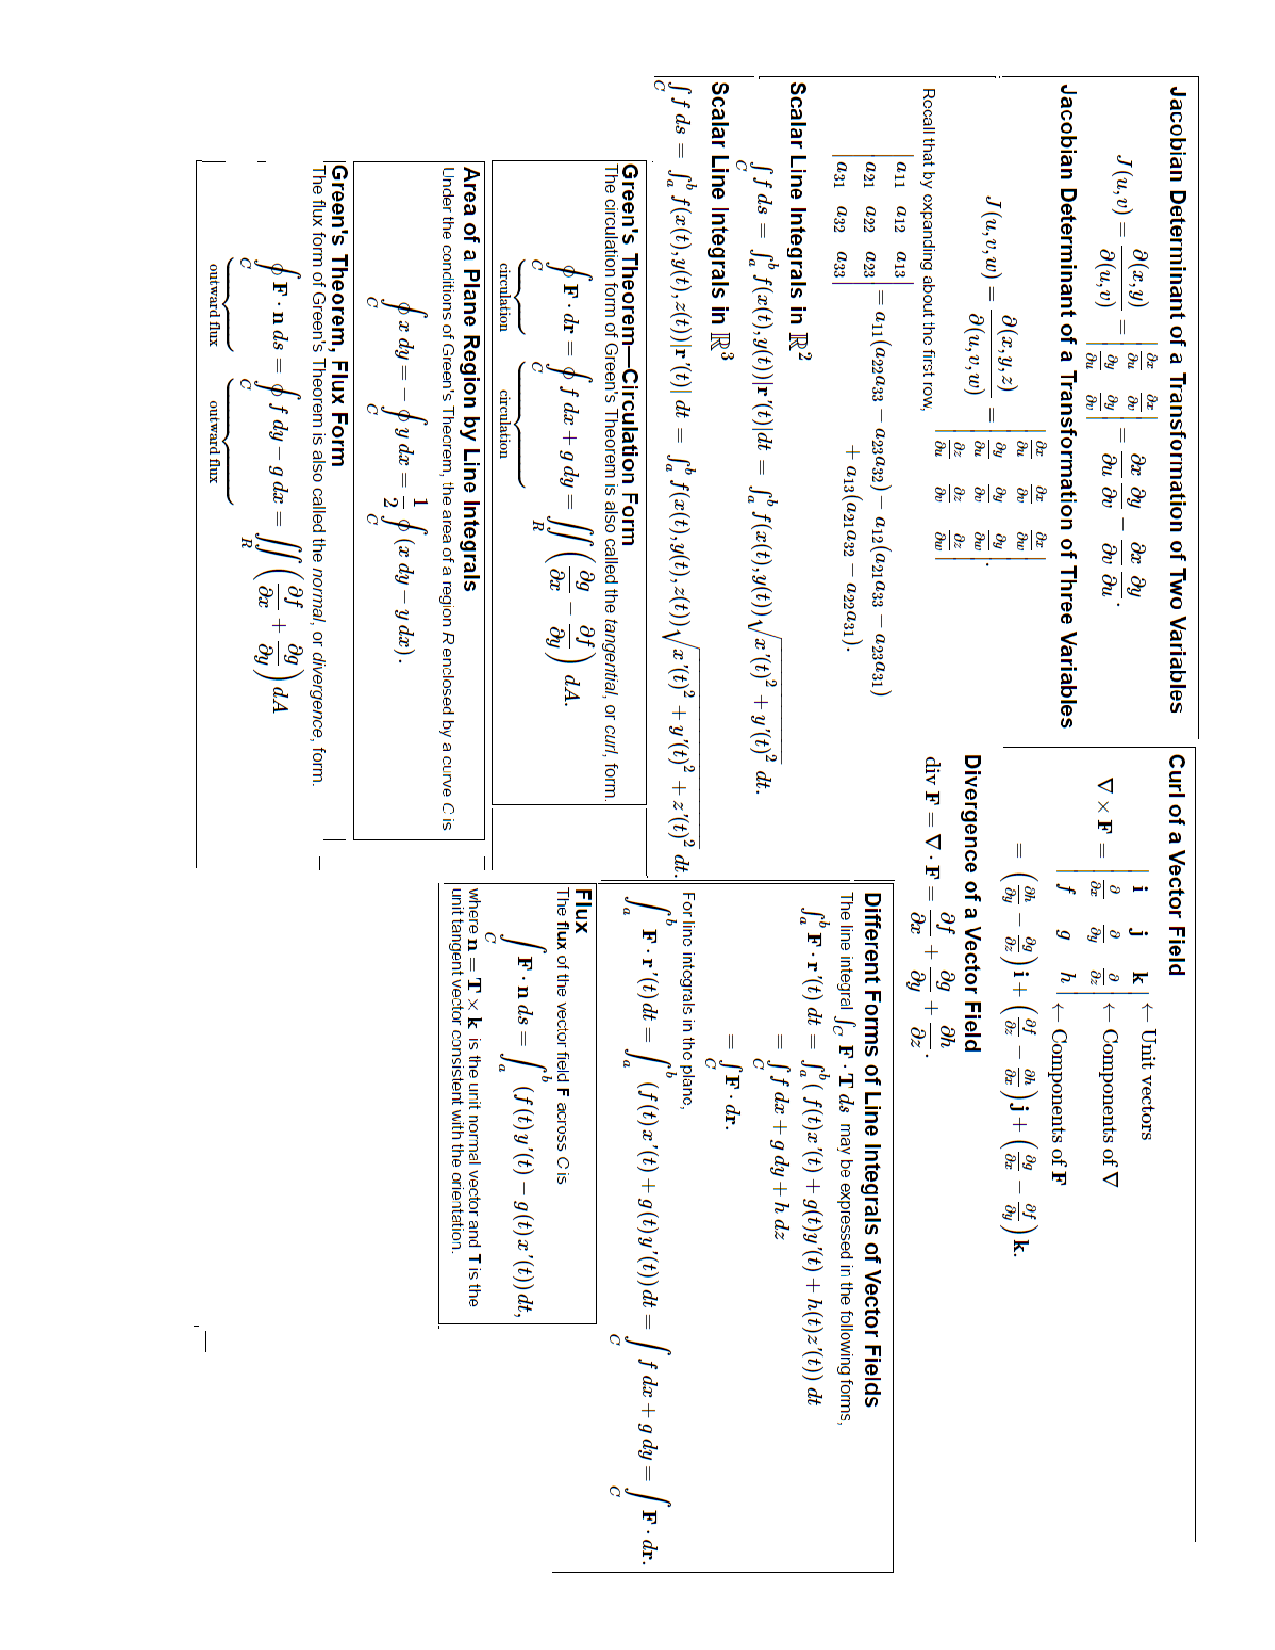
\includegraphics[scale=0.84]{Exam3FormulaSheet.pdf}
\vspace*{\fill}
\end{center}

\newpage

\gradetable
\end{coverpages}

% % % % % % % % % % % % % % % % % % % %
\begin{questions}
\thispagestyle{headandfoot}

% % % % %
\question[16] %{\bf \S13.7 \#47}
Compute the Jacobian, $J(\rho,\varphi,\theta)$, of the following transformation taking Cartesian to spherical coordinates:
\[
x = \rho \sin{\varphi}\cos{\theta} \qquad
y = \rho \sin{\varphi}\sin{\theta} \qquad
z = \rho \cos{\varphi}
\]
You must show your work and simplify.

\newpage

% % % % %
\question[16] %{\bf \S14.4 \#18}
Use Green's Theorem to find the area inside an ellipse with major and minor axes of length 
12 and 8, 
%10 and 9, 
respectively.  In case you need them, the half-angle formulas are $\cos^2x=\frac{1+\cos{2x}}{2}$ and $\sin^2x=\frac{1-\cos{2x}}{2}$.

\newpage

% % % % %
\question %{\bf \S14.5 \#22}
The vector field $\vect F=\langle x,y^2\rangle$, the circle $C$ of radius 2 centered at the origin, and two points $P=(-1,1)$ and $Q=(-1,-1)$, are given in the figure below.

\vspace{-1pc}
\begin{center}
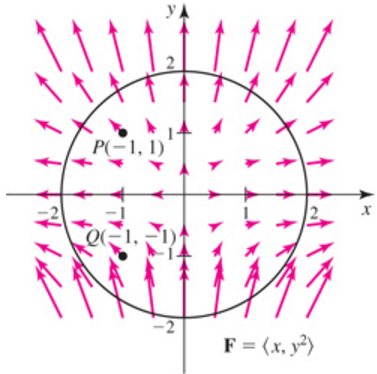
\includegraphics[scale=0.6]{14-5Exam3}
\end{center}

%\vspace{0.5pc}
\begin{parts}
	% % %
	\part[5] Without computing the divergence, does the graph suggest that the divergence is positive or negative at $P$ and $Q$?  Justify your answer.
	\vspace{6pc}
	
	% % %
	\part[5] Compute the divergence of $\vect F$ at $P$ and $Q$ to confirm your answer to part (a).
	\vspace{8pc}
	
	% % %
	\part[3] Label on the graph where the flux across $C$ is outward. 
	\vspace{1pc}
	
	% % %
	\part[8] Is the \textbf{net} outward flux across $C$ positive or negative?  You must justify your answer.
	\vspace{5pc}
\end{parts}

\newpage
% % % % %
\question[] %{\bf \S14.3 \#40}
Let 
$\vect F=\langle 2xyz,x^2z,x^2y\rangle$.
%$\vect F=\langle 8xyz,4x^2z,4x^2y\rangle$.

\vspace{1pc}
\begin{parts}
	\part[8] What is the curl of $\vect F$?
	\vspace{20pc}
	
	% % %
	\part[10] What is the circulation of $\vect F$ along $C$, where $C$ is the closed curve formed by the square whose corners are the points 
	$(1,1)$, $(-1,1)$, $(-1,-1)$, and $(1,-1)$?
	%$(2,2)$, $(-2,2)$, $(-2,-2)$, and $(2,-2)$?
	\vspace{20pc}
\end{parts}

\newpage

% % % % % 
\question[16] %{\bf \S14.2 \#16}
Evaluate the scalar line integral 
$\int_C(x^2+y^3)\ ds$, 
%$\int_C(x^3+y^2)\ ds$, 
where $C$ is the line segment from 
$(0,0)$ to $(5,5)$.
%$(0,0)$ to $(4,4)$.

\newpage

% % % % % 
\question[12] %{\bf \S14.1 \#16} 
Match vector fields (a)-(d) with graphs (A)-(D).

\vspace{1pc}
\begin{parts}
	\part $\vect F=\langle 0,x^2\rangle$
	%\part $\vect F=\langle y,x\rangle$
	\vspace{0.5pc}
	
	\part $\vect F=\langle x-y,x\rangle$
	\vspace{0.5pc}
	
	\part $\vect F=\langle 2x,-y\rangle$
	\vspace{0.5pc}
	
	\part $\vect F=\langle y,x\rangle$
	%\part $\vect F=\langle 0,x^2\rangle$
	\vspace{1pc}	
\end{parts}

\vspace{1pc}
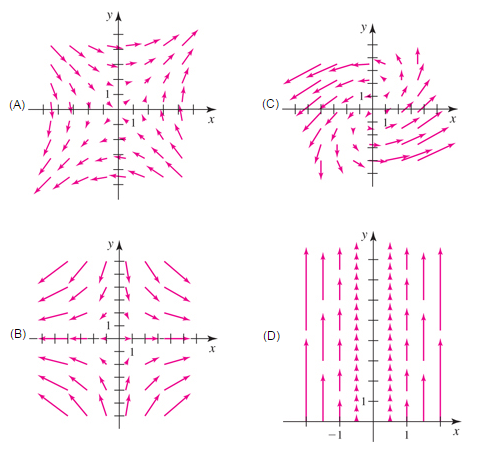
\includegraphics[scale=1.15]{14-1Exam3}
\end{questions}

\end{document}